\documentclass{article}
\usepackage[utf8]{inputenc}
\usepackage{graphicx}
\usepackage{float}
\usepackage{fancyvrb}
\usepackage{amsmath}

\begin{document}

\title{\vspace*{\fill}3D Engine}
\author{João Vieira (a78468) \and José Martins (a78821) \and Miguel Quaresma (a77049) \and Simão Barbosa (a77689)}
\date{%
    Universidade do Minho\\
    Computação Gráfica\\[2ex]%
    \today\vspace*{\fill}
}
\maketitle

\newpage

\tableofcontents

\newpage

\section{Introdução}
O presente relatório servirá de documentação ao processo de desenvolvimento de um motor gráfico 3D que permita a renderização de diversas cenas, nomeadamente a de um sistema planetário, bem como de um gerador de ficheiros que descrevam modelos individuais.

\newpage

\section{Estrutura}
O projecto em mãos é composto por duas componentes principais: 
\begin{description}
    \item [Generator] gerador de ficheiros que descrevem modelos gráficos \textbf{i.e.} um conjunto de vértices(seguidos da sua normal e coordenadas da textura) 
    \item [Engine] motor gráfico que lê ficheiros XML que descrevem determinadas cenas (compostas pelos modelos acima referidos) e renderiza as mesmas
\end{description}

\section{Generator}
Esta componente do projeto é responsável por criar ficheiros que representam modelos/objetos em particular, estes objetos variam de acordo com os argumentos passados pelo utilizador. Este ficheiros contêm informação necessária para o Engine conseguir interpretar e "desenhar" os modelos pretendidos nomeadamente as coordenadas dos vértices que constituem o modelo em questão bem como as normais a estes vértices e ainda as coordenadas correspondentes às texturas. 
O programa está construído de forma a poder responder a pedidos relacionados com 4 objetos:
\begin{itemize}
    \item Um plano em XZ, que recebe como parâmetros x e z
        \begin{verbatim}
exº : ./generator plane 2 4 plane.3d
        \end{verbatim}
    \item Uma caixa, que recebe como parâmetros x, y, z e opcionalmente o número de divisões da mesma
        \begin{verbatim}
exº : ./generator box 2 3 2 box.3d
exº : ./generator box 2 3 2 5 box.3d
        \end{verbatim}
    \item Uma esfera, que recebe o raio, o número de slices e de stacks como parâmetros
        \begin{verbatim}
exº : ./generator sphere 3 10 20 sphere.3d
        \end{verbatim}
    \item Um cone, que recebe o seu raio e altura, bem como o número de slices e stacks como parâmetros
        \begin{verbatim}
exº : ./generator cone 2 4 10 20 cone.3d
        \end{verbatim}
    \item Um conjunto de patches, que recebe o ficheiro com os pontos de controlo e as patches e o nível de tesselagem
        \begin{verbatim}
exº : ./generator bezierPatch teapot.patch 10 teapot.3d
        \end{verbatim}
\end{itemize}
Para além disto, optámos por seguir a sugestão do enunciado e imprimir, na primeira linha dos ficheiros (que contém os pontos a desenhar), o número de vértices que este contém. Isto permitirá alocar o espaço necessário aos \textit{arrays} usados para VBO's por forma a aumentar a performance do motor.

\subsection{Plano (Plane)}
O plano é o modelo mais simples das opções apresentadas, sabendo logo de partida que recebendo apenas os seus dois parâmetros (x e z) apenas é necessário desenhar 2 triângulos para representar o mesmo, ou seja, apenas necessitámos de preencher o ficheiro desejado com 6 pontos, de modo a ser tratado de forma pretendida pelo Engine.

\begin{figure}[H]
\centering
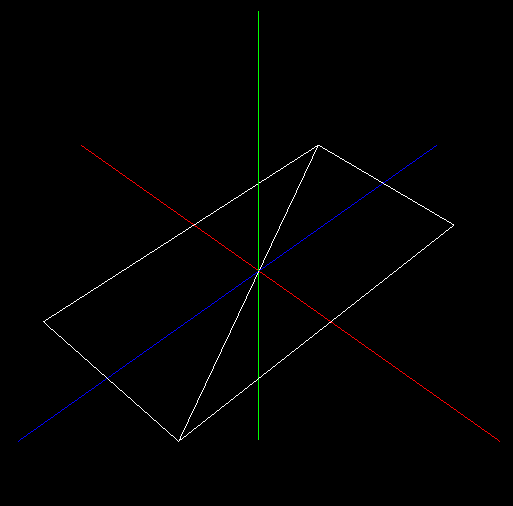
\includegraphics[height=7cm]{plane.png}
\caption{Resultado obtido passando o ficheiro gerado pelo Generator com os parâmetros x=2 e z=4 ao Engine}
\end{figure}

\subsubsection{Em termos matemáticos}
Seja:
\begin{itemize}
    \item x: valor da aresta paralela ao eixo x
    \item z: valor da aresta paralela ao eixo z
\end{itemize}
De modo a desenhar 2 triângulos são necessários 6 pontos:
\begin{itemize}
    \item triângulo 1
        \begin{itemize}
            \item ponto 1: (-x/2,0,-z/2)
            \item ponto 2: (-x/2,0,z/2)
            \item ponto 3: (x/2,0,z/2)
        \end{itemize}
    \item triângulo 2
        \begin{itemize}
            \item ponto 1: (x/2,0,-z/2)
            \item ponto 2: (-x/2,0,-z/2)
            \item ponto 3: (x/2,0,z/2)
        \end{itemize}
\end{itemize}

\begin{figure}[H]
\centering
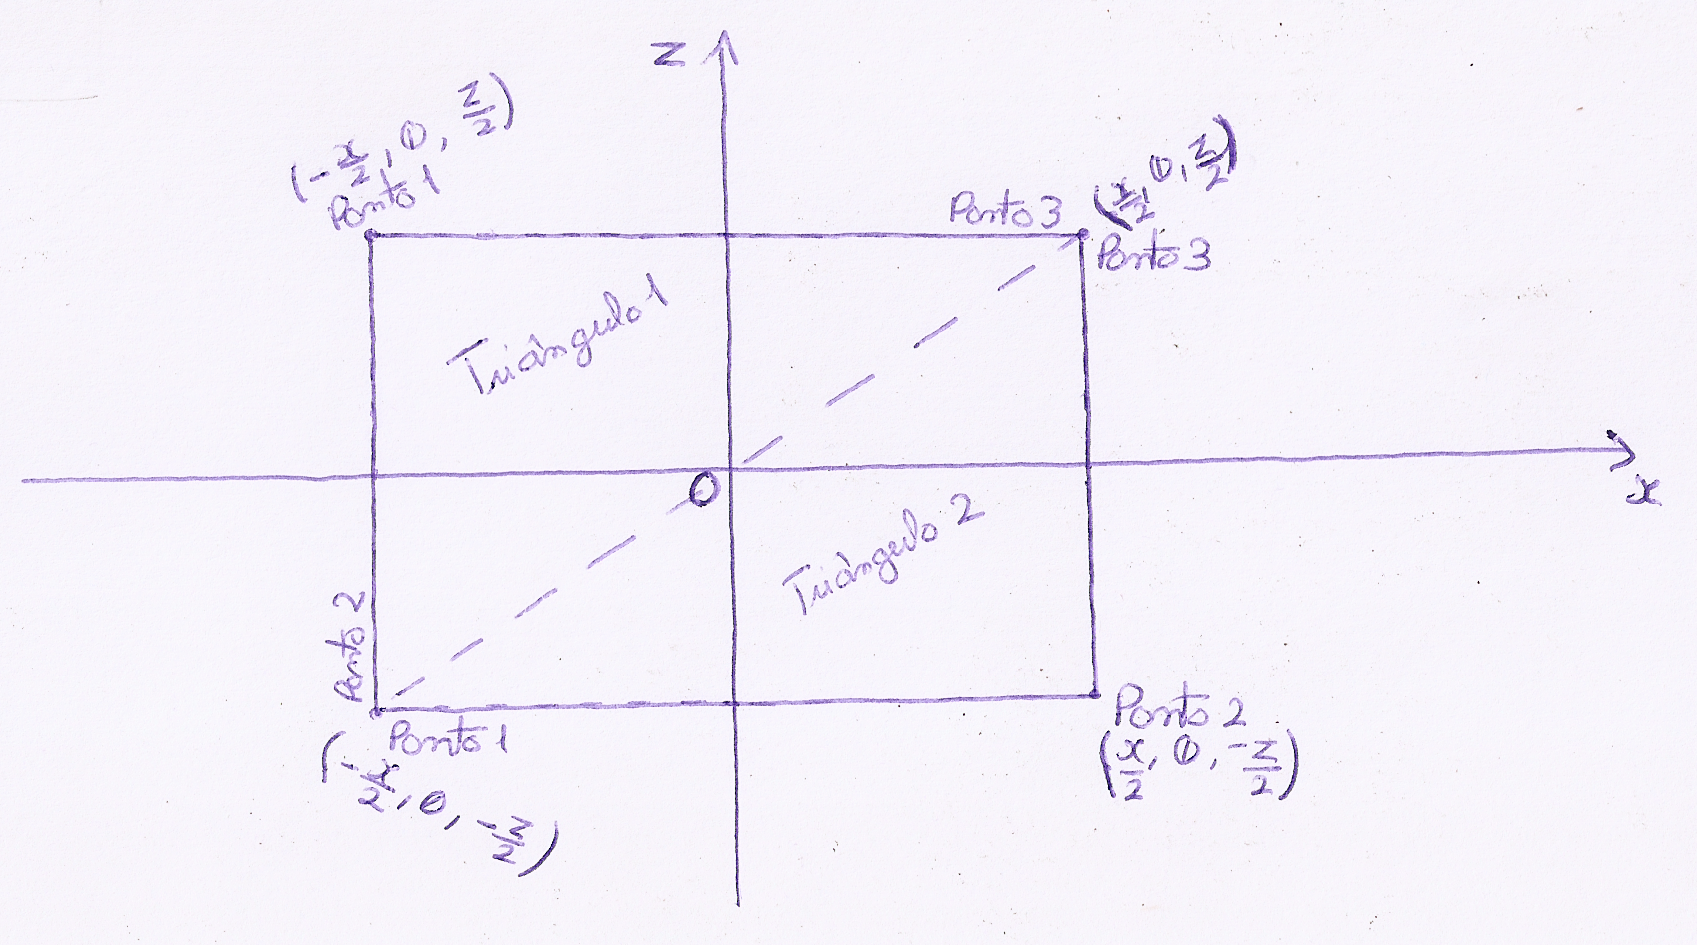
\includegraphics[height=7cm]{planeMath.png}
\end{figure}

\subsubsection{Normais}
Sendo que o plano é o objeto mais simples que o programa oferece, também o cálculo das normais dos pontos do plano é trivial. Sendo que o plano é desenhado em XZ, então a normal dos seus pontos será sempre com x = 0, y = 1 e z = 0.
\begin{verbatim}
normal[0]=0.f; normal[1]=1.f; normal[2]=0.f;
\end{verbatim}

\subsubsection{Texturas}

\subsection{Caixa (Box)}

Na caixa foi feita a assunção de que o seu centro se encontra na origem do gráfico ou seja, no ponto com coordenadas (0,0,0).
Tendo isto em conta, é-nos útil dividir os parâmetros recebidos das dimensões pretendidas por 2, sendo assim utilizados esses mesmos valores para cada um dos pontos positivos e negativos do eixo em causa.
Interpretamos as divisões opcionais da caixa (d) como sendo utilizadas para dividir as faces laterais da caixa em d divisões (no eixo y), e também em d divisões nas faces inferiores e superiores (no eixo x).
Tendo uma caixa 6 faces, e considerando que cada face é um paralelogramo cujos lados formam um ângulo de 90º entre si, é fácil calcular qual o número de pontos necessários a imprimir para ser possível desenhar o modelo:
\begin{itemize}
    \item 1 paralelogramo cujos lados formam um ângulo de 90º entre si é desenhado recorrendo a 2 triângulos
    \item 1 triângulo é desenhado recorrendo a 3 pontos
    \item Logo, cada paralelogramo cujos lados formam um ângulo de 90º entre si necessita de 6 pontos
    \item Com a componente opcional das divisões, cada face passa assim a ter d paralelogramos cujos lados formam um ângulo de 90º entre si.
    \item Ou seja, nº de pontos total = (2 * d + 4 * d) * 6
\end{itemize}
O processo com as divisões é simples, por exemplo, nas faces laterais da caixa, declaramos 2 variáveis y1 e y2 (sendo neste caso as divisões feitas no eixo y), começamos por calcular a variação em altura que cada divisão tem (var\_y = y/d) e atribuímos os valores:
\begin{itemize}
    \item y1 = -y;
    \item y2 = -y + var\_y;
\end{itemize}
A partir daqui e com a utilização de um ciclo com a inicialização da uma variável i a 0 e enquanto a mesma for menor que o número de divisões pretendidas d, utilizamos as funções criadas por nós para obter os pontos dos paralelogramos cujos lados formam um ângulo de 90º entre si/divisões das faces da caixa progressivamente (neste caso, faceYZ() e faceXY()), incrementando o valor de i, e aumentando em var\_y os valores de y1 e y2 no fim de cada iteração.

\begin{figure}[H]
\centering
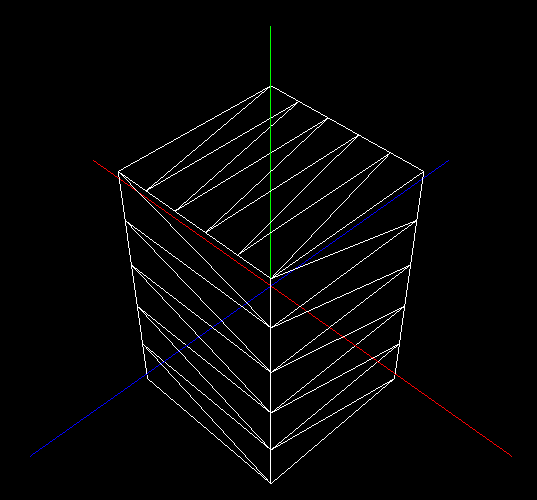
\includegraphics[height=7cm]{box.png}
\caption{Resultado obtido passando o ficheiro gerado pelo Generator com os parâmetros correspondentes a uma box com 5 divisões ao Engine}
\end{figure}

\subsubsection{Em termos Matemáticos}
Não considerando divisões, ou seja apenas 2 triângulos por face, seja:
\begin{itemize}
    \item xI: valor das arestas paralelas ao eixo x (input 1)
    \item yI: valor das arestas paralelas ao eixo y (input 2)
    \item zI: valor das arestas paralelas ao eixo z (input 3)
\end{itemize}
Visto que a Box tem de estar centrada na origem estes valores são divididos por 2 de modo a facilitar os cálculos:
\begin{itemize}
    \item x=xI/2
    \item y=yI/2
    \item z=zI/2
\end{itemize}
Com base na seguinte figura:
\begin{figure}[H]
    \centering
    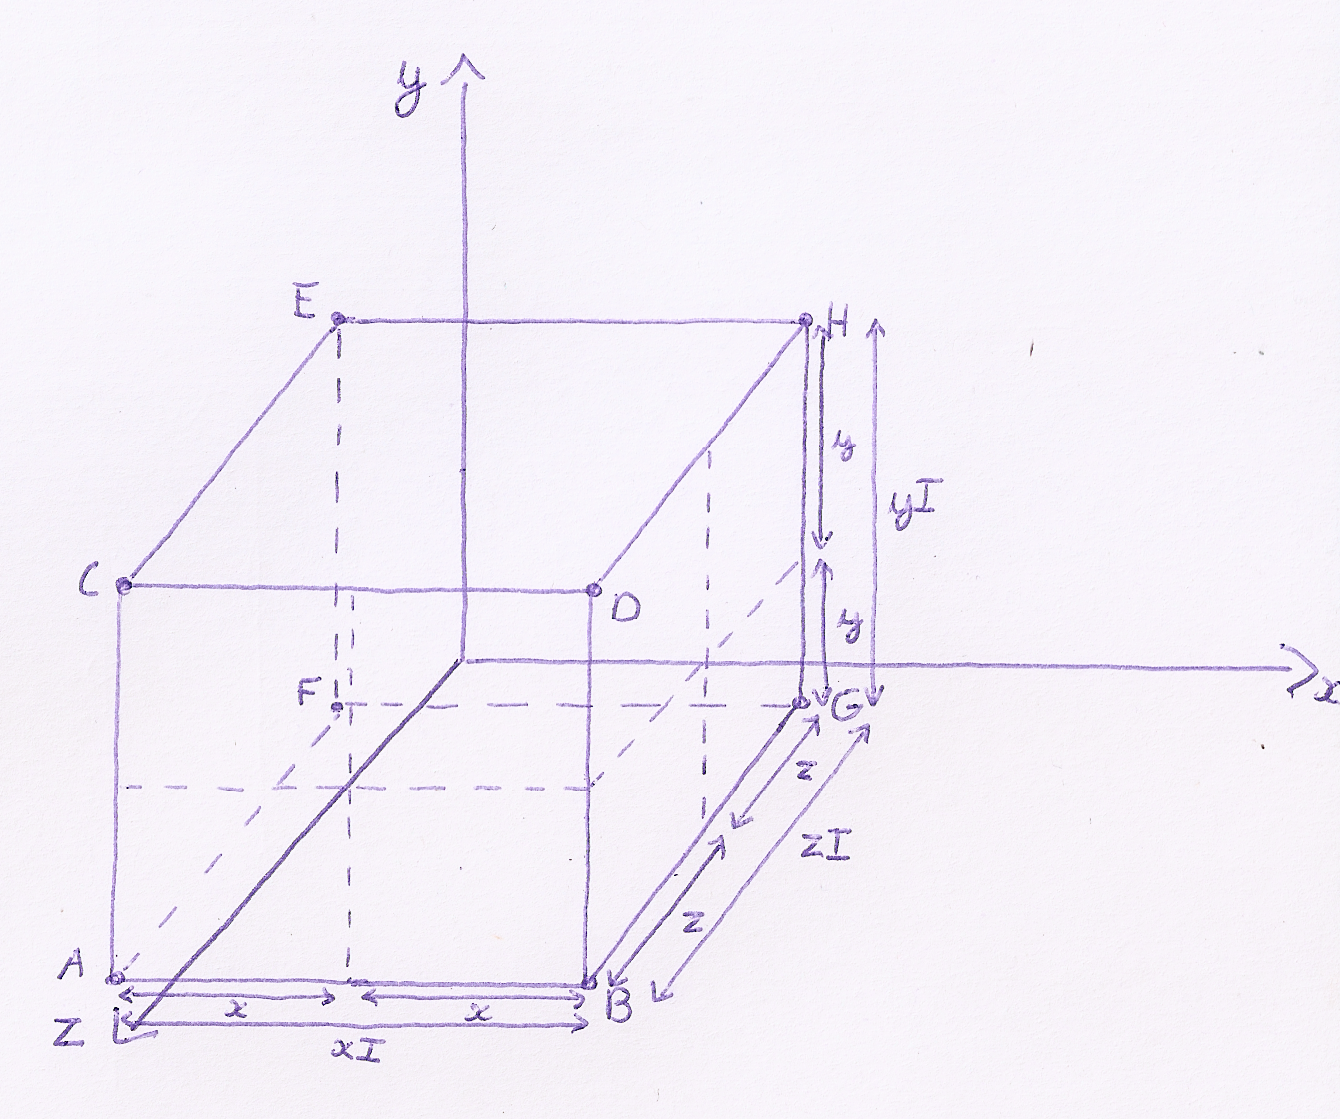
\includegraphics[height=10cm]{boxMath1.png}
\end{figure}
Os vértices da box são:
\begin{itemize}
    \item A = (-x,-y,z)
    \item B = (x,-y,z)
    \item C = (-x,y,z)
    \item D = (x,y,z)
    \item E = (-x,y,-z)
    \item F = (-x,-y,-z)
    \item G = (x,-y,-z)
    \item H = (x,y,-z)
\end{itemize}
Consideremos agora apenas as faces ABCD e EFGH:
\begin{figure}[H]
    \centering
    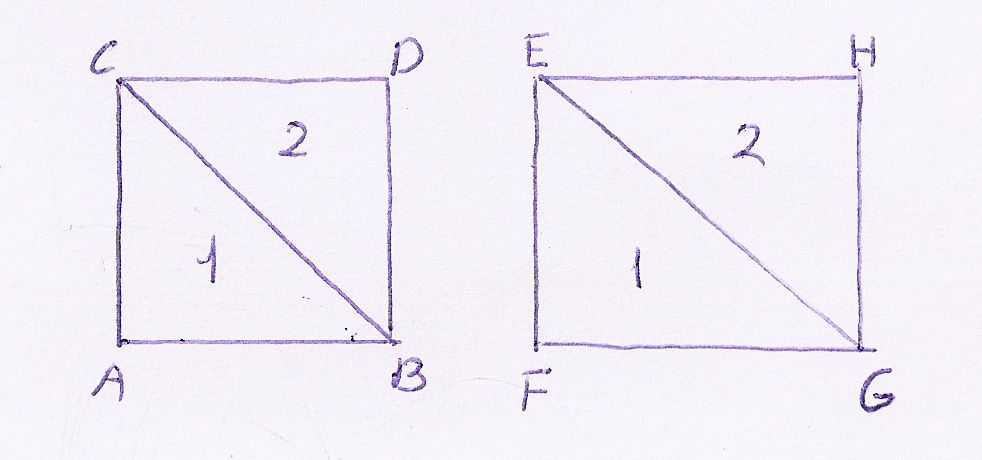
\includegraphics[height=5cm]{boxMath2.png}
\end{figure}
Para desenhar as faces(2 triângulos por cada face) as ordens dos pontos seria, por exemplo:
\begin{figure}[H]
    \centering
    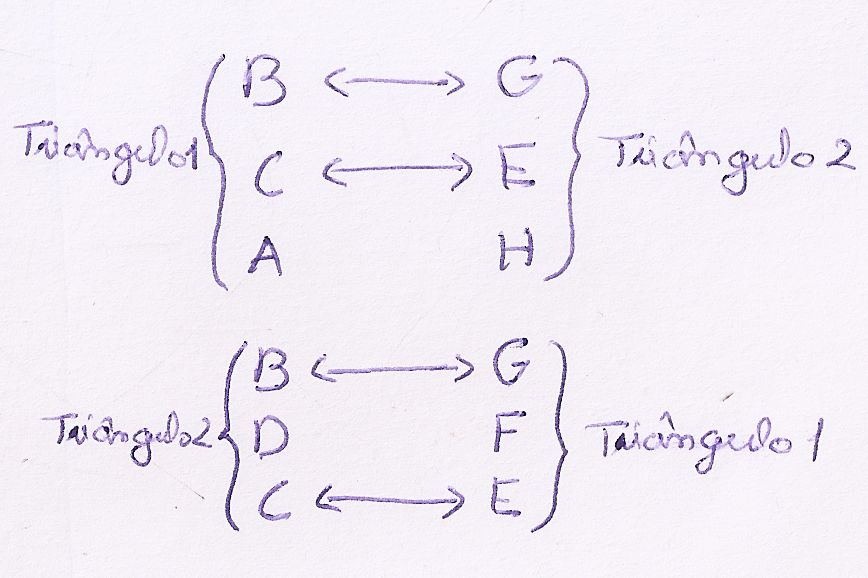
\includegraphics[height=5cm]{boxMath3.png}
\end{figure}
Entre os pontos B e G e entre os pontos C e E apenas é alterado a coordenada z que é simétrica. Sendo assim, na função faceXY podemos (chamando duas vezes a função, uma com zParâmetro=z e outra com zParâmetro=-z) desenhar as duas faces sendo que, os pontos B e G são desenhados pela mesma expressão(x,-y,zParâmetro) e os C e E também(-x,y,zParâmetro). Para os outros pontos é usado um if e consoante o valor de z é desenhado os pontos correspondentes:
\begin{verbatim}
//triângulo 1 da face ABCD(z>0) ou triângulo 2 da face EFGH(z<0)
(-x,y,zParâmetro) // desenhar C ou E
(x,-y,zParâmetro) //desenhar B ou G
if(z>0) (x,y,zParâmetro) //desenhar D
else (-x,-y,zParâmetro) //desenhar F

//triângulo 2 da face ABCD(z>0) ou triângulo 1 da face EFGH(z<0)
(x,-y,zParâmetro) //desenhar B ou G
(-x,y,zParâmetro) // desenhar C ou E
if(z>0) (-x,-y,zParâmetro) //desenhar A
else (x,y,zParâmetro) //desenhar H
\end{verbatim}
Isto é aplicado às outras faces mudando a coordenada simétrica:
\begin{itemize}
    \item faces paralelas a YZ: coordenada x (função faceYZ)
    \item faces paralelas a XZ: coordenada y (função faceXZ) 
\end{itemize}

Consideremos agora as divisões:
\newline
O processo por detrás das divisões das faces da caixa passa por dividir cada uma das faces em N retângulos, sendo este N o número de divisões pretendidas.

\begin{figure}[H]
\centering
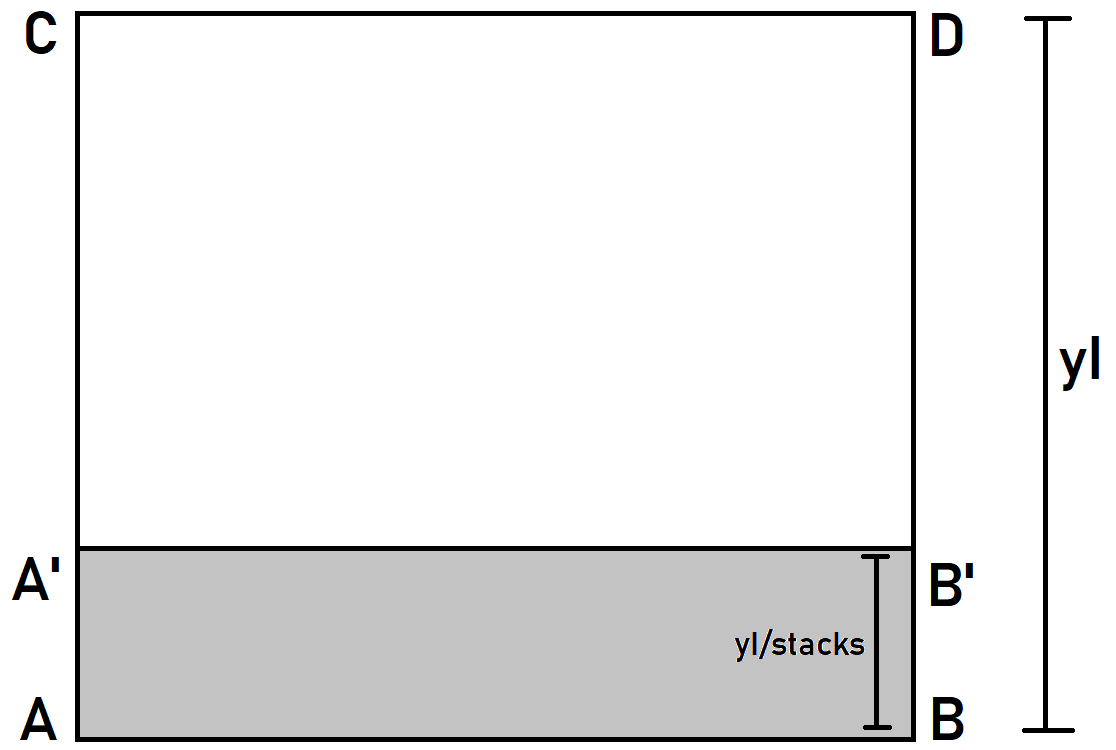
\includegraphics[height=7cm]{caixaStacks1.png}
\end{figure}

Seguindo a face [A B D C] enunciada em cima, desta forma, começamos por desenhar o retângulo [A B B' A'] através da função \textit{faceXY}(visto que a mesma desenha 2 triângulos que formam um paralelogramo cujos lados formam 90º entre si), que representa a primeira \textit{stack} da face em causa, sendo que $|$yA'-yA$|$=$|$yB'-yB$|$=yI/stacks (sendo por exemplo yA o valor da coordenada y no ponto A').

\begin{figure}[H]
\centering
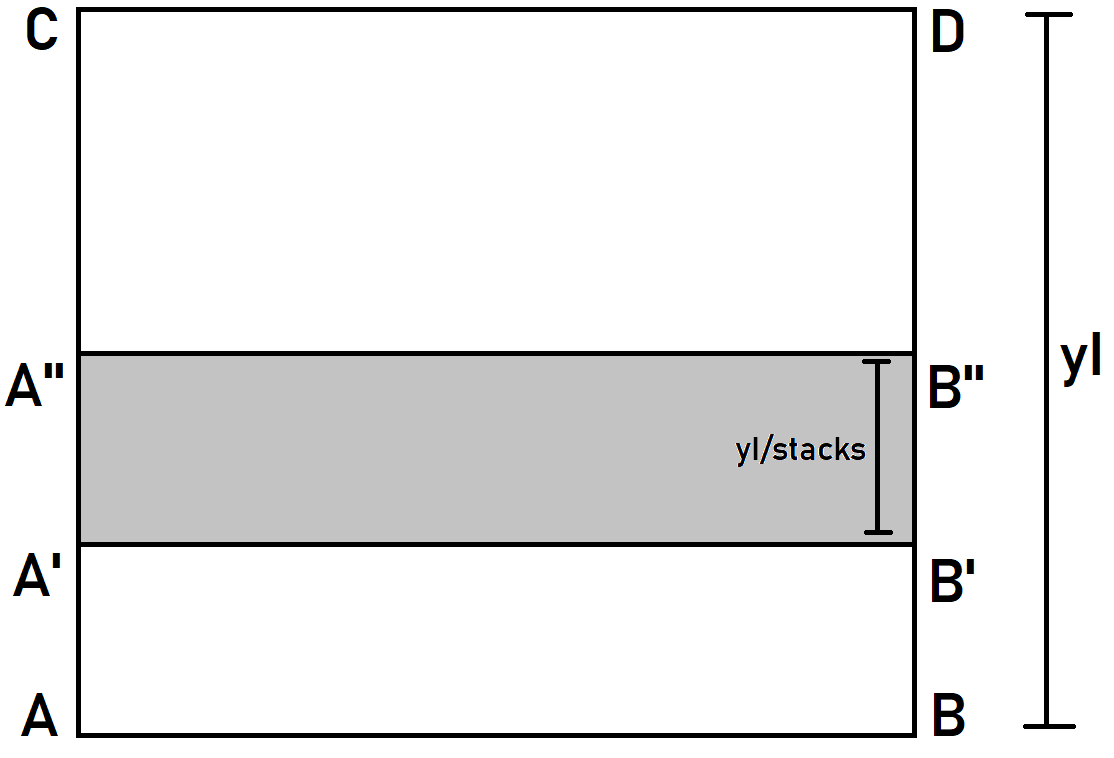
\includegraphics[height=7cm]{caixaStacks2.png}
\end{figure}

Na próxima iteração passamos a desenhar o retângulo [A' B' B'' A''] e por aí adiante, até concluirmos o números de \textit{stack's} que queremos obter.
\newline
Nesta face, o eixo que faz variar as divisões é o y, já no caso da face superior e da inferior este eixo passa a ser o x, mas seguindo sempre a mesma teoria.

\subsubsection{Normais}
Para calcular as normais dos pontos que representam uma caixa, é necessário ter em atenção a face da caixa a que determinado ponto pertence.\\
Desta forma, se um ponto pertencer a uma face no plano XZ, então o vetor da normal tem como valores x = 0 e z = 0, sendo que o valor de y depende da coordenada y deste mesmo ponto, se este valor for maior que zero, então o valor de y no vetor normal é 1 (face superior do cubo), caso contrário este y toma como valor -1 (face inferior).\\
Se o ponto pertencer a uma face no plano YZ, então no vetor normal deste ponto y = 0 e z = 0, enquanto que x toma o valor de 1, caso o valor da coordenada y do ponto seja superior a 0, e toma o valor de -1 no caso contrário.\\
Por fim, quanto à face XY, é sabido que no vetor normal x = 0 e y = 0, e o valor de z pode também tomar o valor de 1 ou -1, para o caso de o valor da coordenada z do ponto em causa ser superior ou inferior a 0.

\subsubsection{Texturas}

\subsection{Esfera (Sphere)}
A esfera é o modelo mais complexo dos envolvidos. Neste modelo, mais uma vez, o centro foi colocado na origem. O número de vértices necessários para a esfera é calculado da seguinte maneira:
\begin{enumerate}
    \item a esfera é formada por y \textit{stacks}
    \item cada \textit{stack} é formada por x \textit{slices}
    \item cada \textit{slice} possui 2 triângulos que formam a parede que liga à \textit{stack} superior
    \item cada triângulo tem 3 pontos
    \item nro. total de pontos=6*\textit{slices}*(2*\textit{stacks}-1)
\end{enumerate}

O cálculo dos pontos que forma as laterais da esfera e do cone é feita com recurso à função:
\begin{Verbatim}
    void genWalls(int fd, int sliceCount, float radius, float curRadius, 
        float y, float angle, float delta, float top,int tpbt, float height)
\end{Verbatim}

Para tal esta calcula os dois triângulos que formam a superfície de cada uma das figuras (cone e esfera).
\begin{figure}[H]
    \centering
    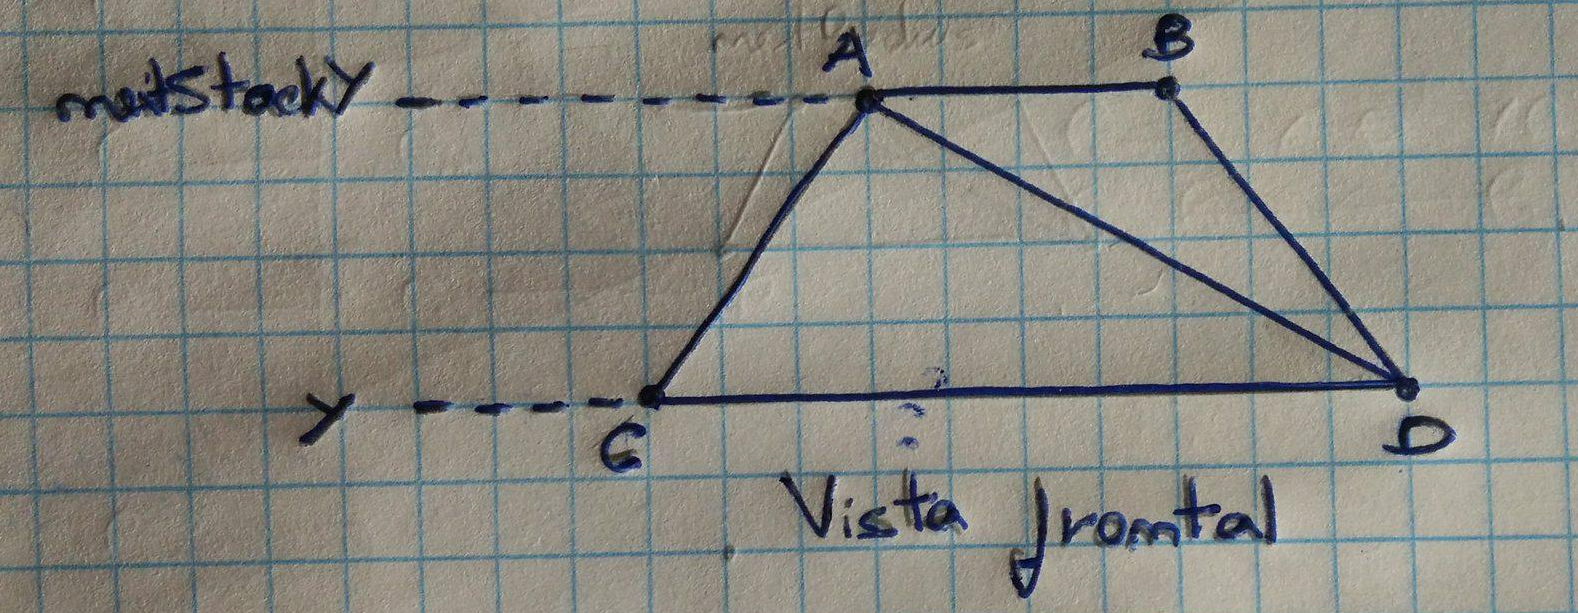
\includegraphics[height=4cm]{genWallsDemo.jpg}
    \caption{Superfície desenhada por cada iteração do loop da função \texttt{genWalls}}
\end{figure}

Tendo em conta as seguintes assunções:
\begin{itemize}
    \item \texttt{nextRadius} raio da \textit{stack} seguinte
    \item \texttt{nextStackY} valor da coordenada y para os pontos da \textit{stack} seguinte
    \item \texttt{curRadius} raio da \textit{stack} atual
    \item \texttt{y} valor da coordenada y da \textit{stack} atual
    \item \texttt{angle} amplitude de cada \textit{slice} que compõem a \textit{stack}
\end{itemize}
segue que:
\\

$A=(nextRadius*\sin(curAngle),nextStackY,nextRadius*\cos(curAngle))$

$B=(nextRadius*\sin(curAngle+angle),nextStackY,nextRadius*\cos(curAngle+angle))$

$C=(curRadius*\sin(curAngle),y,curRadius*\cos(curAngle))$

$D=(curRadius*\sin(curAngle+angle),y,curRadius*\cos(curAngle+angle))$


(\textbf{conf.} \ref{PolarCoordinates}-Coordenadas Polares)
\\

O parâmetro \texttt{tpbt} é usado para indicar se a \textit{stack} a ser desenhada pertence ao extremo superior(1), extremo inferior(-1) ou se é uma \textit{stack} intermédia por forma a impedir que nos extremos sejam calculados o dobro dos pontos necessários. O parâmetro \texttt{top} é usado para determinar se a função está a ser chamada para gerar parte da esfera ou parte do cone para poder realizar a normalização quando se tratar do primeiro caso, sendo também usado, no caso da esfera, para determinar se está a ser calculada a metade superior ou a metade inferior.

Inicialmente são calculados os pontos que formam a metade superior da esfera. Visto tratar-se de uma esfera procedemos à normalização dos pontos antes de os escrevermos no ficheiro de configuração. A normalização tem como objetivo manter a distância dos triângulos a serem desenhados em relação à origem (\textbf{i.e} centro da esfera) igual ao raio mantendo, no entanto, o ângulo entre estes.

\begin{figure}[H]
    \centering
    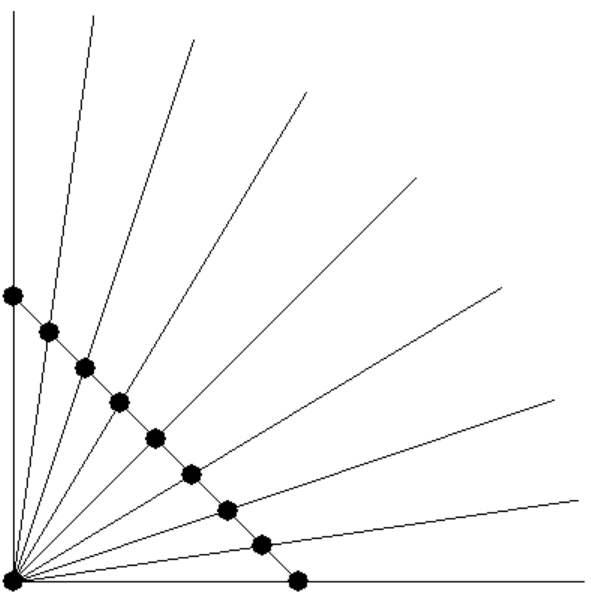
\includegraphics[height=4cm]{beforeNorm.png}
    \caption{Pré-normalização}
\end{figure}

\begin{Verbatim}[fontsize=\small]    
    float dist=sqrt(cur[0]*cur[0]+cur[1]*cur[1]+cur[2]*cur[2]);
      
    cur[0]=(cur[0]*radius)/dist;
    cur[1]=(cur[1]*radius)/dist;
    cur[2]=(cur[2]*radius)/dist;
\end{Verbatim}

\begin{figure}[H]
    \centering
    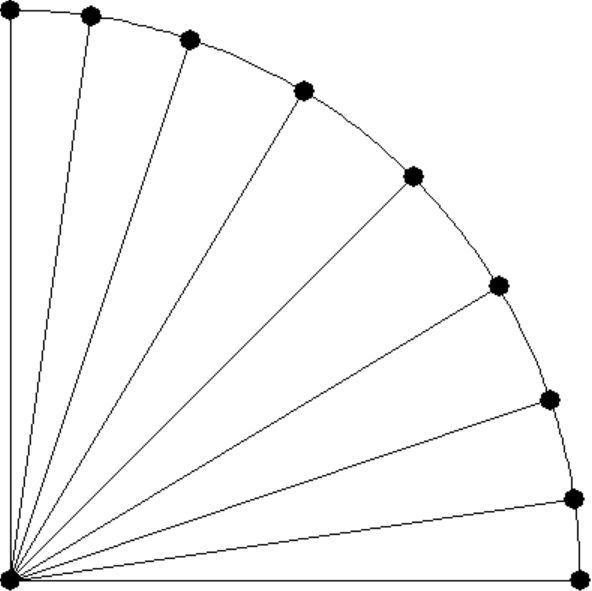
\includegraphics[height=4cm]{afterNorm.png}
    \caption{Pós-normalização}
\end{figure}

Este mesmo processo é depois aplicado à metade inferior da esfera, permitindo assim a obtenção de uma esfera completa. Uma particularidade desta figura é o facto de não ser necessário calcular os pontos correspondentes a cada uma das \textit{stacks} já que estas não são visíveis do exterior, como tal apenas são calculados os pontos referentes às paredes.

\begin{figure}[H]
    \centering
    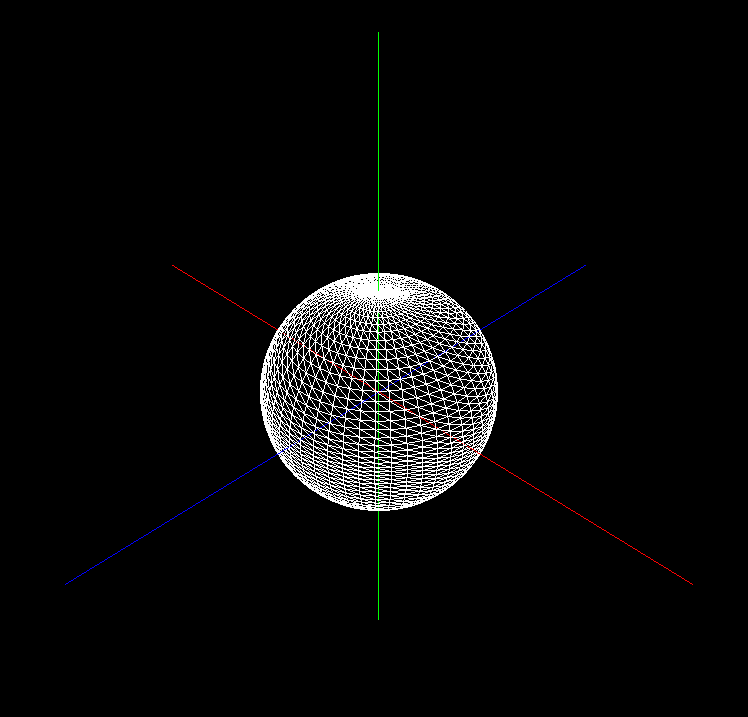
\includegraphics[height=7cm]{sphereFinal.png}
    \caption{Resultado obtido usando como parâmetros 1 50 50}
\end{figure}

\subsubsection{Normais}
Para o cálculo das normais nos pontos de uma esfera, apenas é necessário ter em conta que o vetor normal de um determinado ponto numa esfera toma o valor das coordenadas desse mesmo ponto subtraindo as coordenadas do centro da mesma.\\
Desta forma, como no problema em questão, o centro das esferas desenhadas toma sempre o valor da origem do gráfico (0,0,0), o vetor normal em todos os pontos de uma esfera é o próprio valor das coordenadas do mesmo.

\subsubsection{Texturas}

\subsection{Cone (Cone)}
O cone, tal como a esfera, é um dos modelos mais complexos, tanto em termos de cálculo dos pontos necessários como também da quantidade dos mesmos. No caso do cone, o centro da base foi colocado na origem do referencial. O número de pontos necessário à configuração do modelo do cone é calculado da seguinte maneira:
\begin{enumerate}
    \item o número de pontos da superfície lateral é calculado da mesma maneira que o número de pontos usados para a esfera(6*(\textit{stacks}-1)*\textit{slices})
    \item a base é constituída por s \textit{slices}
    \item cada \textit{slice} (da base) é constituída por 3 pontos
    \item nro. total de pontos=6*\textit{slices}*\textit{stacks}
\end{enumerate}

Como já foi referido, a função \texttt{genWalls} é usada para calcular os pontos que compõem a superfície lateral do cone. No entanto, visto que no cone não existe a noção de raio, não é necessário normalizar os pontos, isto é conseguido através do parâmetro \texttt{deltaH} que corresponde à variação no eixo dos yy entre \textit{stacks} consecutivas e que, no caso da esfera, é igual ao valor de deltaR (variação do raio entre \textit{stacks} consecutivas) sendo por isso passado um valor menor ou igual a 0 caso se trate da metade superior ou inferior respetivamente, permitindo assim a seguinte condição:

\begin{Verbatim}
    else if(top>0.f) nextStackY=y+top;
    ...
    if(top<=0.f)curP=normalize(curP,radius);
\end{Verbatim}

Por fim é gerada a base do cone que consiste em numa aproximação a um círculo por meio de s \textit{slices}, cada uma delas um triângulo. Também neste caso são usadas coordenadas polares (\textbf{conf.} \ref{PolarCoordinates}) para calcular os pontos que constituem cada \textit{slice}.

\begin{figure}[H]
    \centering
    
\includegraphics[height=4cm]{circleStack.png}
    \caption{Aproximação de \textit{stack} a círculo}
\end{figure}


\begin{figure}[H]
    \centering
    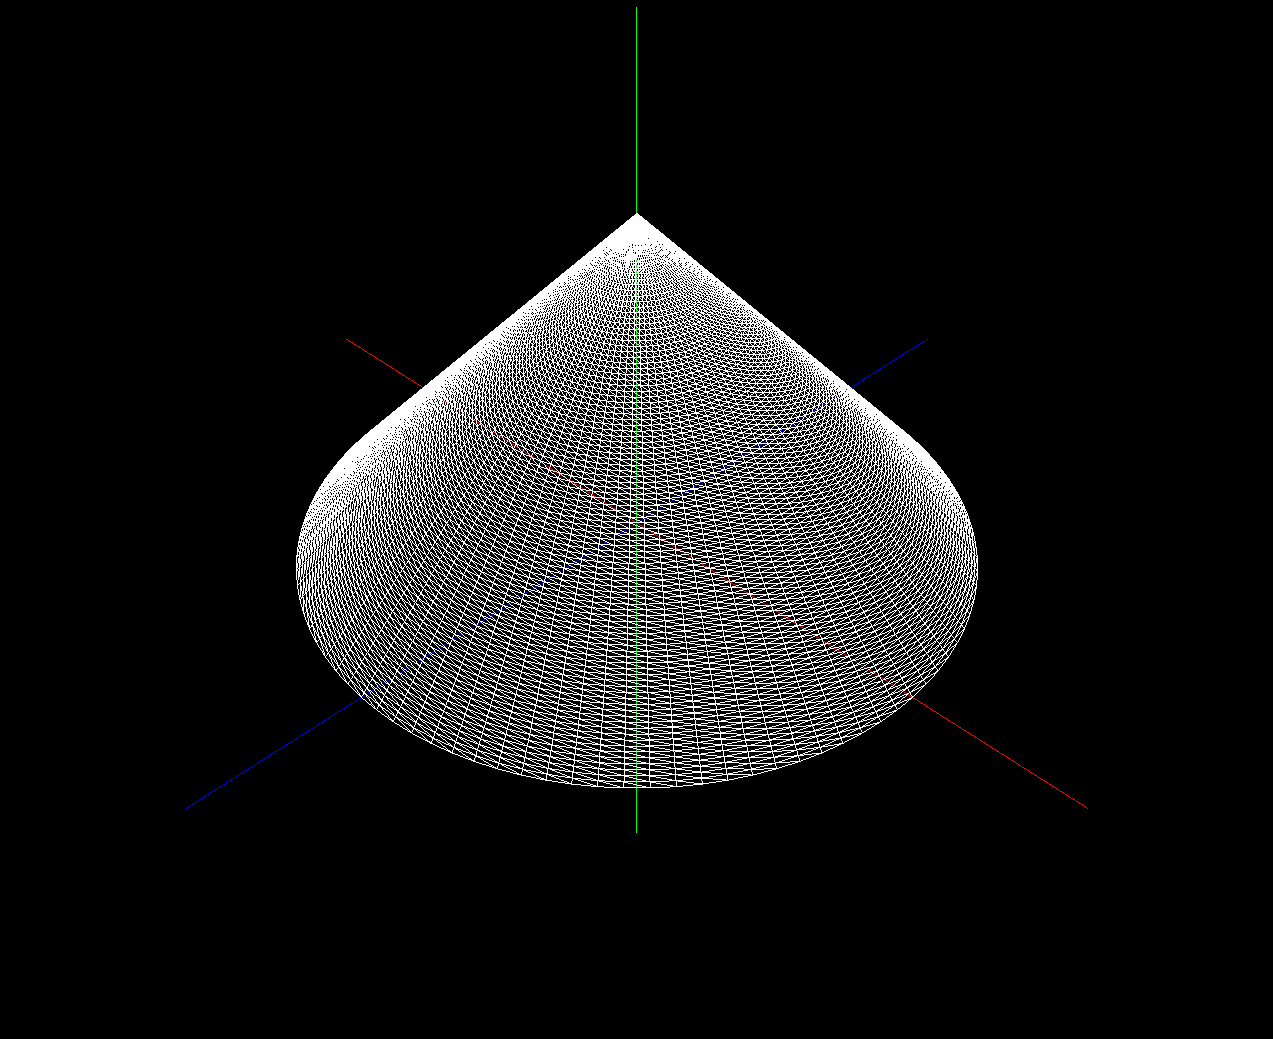
\includegraphics[height=7cm]{coneFinal.png}
    \caption{Resultado obtido usando como parâmetros 2 2 100 100} 
\end{figure}

\newpage

\subsubsection{Normais}

\subsubsection{Texturas}

\subsection{Bezier Patches}
De modo a gerar no generator os triângulos correpondentes à figura presente num ficheiro \textit{.patch} inicialmente é necessário carregar os valores presentes no mesmo para memória daí a existência de \textit{getNumber} que obtém o número de \textit{Patches} ou o número de \textit{Control Points}, de \textit{getPatches} que guarda os índices dos pontos de controlo e por fim de \textit{getControlPoints} que guarda os pontos de controlo.

Após esta fase de recolha de dados, imprime-se no ficheiro de \textit{output} o número de pontos que irão ser gerados: $numPatches*(tesselationLevel-1)*(tesselationLevel-1)*6$, em que \textit{tesselationLevel} é o número de tesselagem passado como parâmetro, que \textit{numPatches} é o número de \textit{patches}, que 6 deriva do facto de que para cada 2 triângulos são necessários 6 pontos, e por fim é multiplicado pelo número de secções(2 triângulos) que irão existir em cada patch ($(tesselationLevel-1)*(tesselationLevel-1)$) visto que o que será gerado é uma malha destas secções na superficie delimitada pelos pontos extremos de controlo (os 4 pontos de controlo presentes em cada canto da matriz com os pontos de controlo).

De seguida para cada \textit{patch} é recolhido os pontos de controlo a partir dos índices de cada \textit{patch} com a função \textit{getPatchPoints} para logo de seguida ser calculada a matriz constante $RES=M*CP*M^T$, sendo CP a matriz dos pontos de controlo recolhidos anteriormente, na função \textit{mMultCpMultM}. Portanto com a matriz resultante (RES) é calculado os ``novos'' pontos de modo a gerar os triângulos a partir dos mesmos. 

Tendo em conta que u e v só podem variar de 0 a 1 e que recebemos como parâmetro o nivel de tesselagem (\textit{tesselationLevel}) que tem de ser no mínimo 4, caso em que os pontos resultantes são os próprios pontos de controlo, é calculado cada ponto com a função \textit{calcPoint} sendo guardado em \textit{points} para posterior criação de triângulos. Esta função (\textit{calcPoint}) é chamada num loop duplo que, varia v entre 0 e 1 aumentando v em $1/(tesselationLevel-1)$ em cada iteração no loop externo e no loop interno u varia entre 0 e 1 aumentado u também em $1/(tesselationLevel-1)$ em cada iteração. 

A função calcPoints calcula a posição do ponto atravês da fórmula de Bezier: $\begin{bmatrix} u^3 & u^2 & u & 1 \end{bmatrix}*RES*\begin{bmatrix} v^3 \\ v^2 \\ v \\ 1 \end{bmatrix}$
em que como visto anteriormente $RES=M*CP*M^T$, com CP sendo os pontos de controlo.

Por fim sao percorridos os pontos guardados em \textit{points} de modo a criar os triângulos:
\begin{verbatim}
for(int t=0; t<tL-1; t++){
    for(int q=0; q<tL-1; q++){
        printLine(fd,array,points[t][q][0],points[t][q][1],points[t][q][2]);
        printLine(fd,array,points[t][q+1][0],points[t][q+1][1],points[t][q+1][2]);
        printLine(fd,array,points[t+1][q][0],points[t+1][q][1],points[t+1][q][2]);

        printLine(fd,array,points[t+1][q][0],points[t+1][q][1],points[t+1][q][2]);
        printLine(fd,array,points[t][q+1][0],points[t][q+1][1],points[t][q+1][2]);
        printLine(fd,array,points[t+1][q+1][0],points[t+1][q+1][1],points[t+1][q+1][2]);
    }
}
\end{verbatim}

\subsubsection{Normais}

\subsubsection{Texturas}

\newpage

\section{Engine}
A componente Engine é fundamental no projeto visto que é esta que realiza a renderização das cenas descritas em ficheiros XML com uma sintaxe predefinida.
Para que isto seja possível recorremos às seguintes bibliotecas:
\begin{description}
    \item [Libxml2] Parser XML utilizado devido à sua familiaridade com o mesmo bem como simplicidade
    \item [OpenGL] Usado para desenhar sendo a sua utilização justificada por ser open-source e devido à presença de boa documentação
    \item [Glut] Biblioteca de "colagem" entre OpenGL e SO
    \item [Glew] Necessário para a utilização de VBO's
\end{description}
Portanto, com recurso ao mesmo (libxml2) obtemos do ficheiro XML e pela ordem apresentada no mesmo, os ficheiros em que cada um possui pontos/normais/coordenadas de textura referentes a um objeto tridimensional, sendo estes ficheiros possíveis de ser gerados pelo generator atrás referido. 
Para guardar estes pontos é utilizado uma estrutura (Points) que é uma lista ligada, sendo cada elemento constituído por:
\begin{itemize}
    \item Um array com todas as coordenadas dos pontos disponibilizados por determinado ficheiro
    \item Um array com todas as normais dos pontos
    \item Um array com as coordenadas de textura
    \item O id da textura a usar
    \item Um array com as cores do objeto (ver-se-á mais à frente na secção Materials a sua necessidade)
    \item O número de pontos que essas coordenadas "geram"
    \item Um apontador para a próxima estrutura (ficheiro seguinte)
\end{itemize}
De modo a desenhar os pontos/normais/coordenadas de textura correspondentes aos presentes nos ficheiros e agora também nos arrays, é usado VBO's facilitando e melhorando a performance. As figuras são desenhadas por um conjunto de triângulos, e, como tal, a cada 3 pontos é desenhado um. 

\subsection{Câmeras}
Foi implementado, recorrendo a coordenadas polares, a possibilidade de mover a câmara:
\begin{itemize}
    \item Rodar horizontalmente à esquerda: tecla seta esquerda
    \item Rodar horizontalmente à direita: tecla seta direita
    \item Rodar verticalmente para cima: tecla seta cima
    \item Rodar verticalmente para baixo: tecla seta baixo
    \item Aproximar: tecla 'w'
    \item Afastar: tecla 's'
\end{itemize}
Para além disso, carregando na tecla 'm' é alterado consecutivamente o modo de display dos polígonos, alternando entre FILL (a cheio), LINE (em linhas) e POINT (apenas pontos).

Para além disso, optamos por implementar o modo de \textit{First Person Camera} (FPC). Este sistema de visualização permite observar os modelos construídos de um modo diferente e confere um maior realismo ao \textit{Engine}, tornando o programa um pouco mais completo. A implementação desta mesma câmara foi realizada de modo a que ao clicar na tecla \textit{'t'} se possa alterar entre o modo de vista por nós já implementado anteriormente e este novo modo.
\newline
Dentro deste modo de visualização, utilizamos as teclas:
\begin{itemize}
    \item \textit{'w'} para mover a câmara para a frente
    \item \textit{'s'} para mover a câmara para trás
    \item \textit{'a'} para mover a câmara para a esquerda
    \item \textit{'d'} para mover a câmara para a direita
    \item setas direita e esquerda para efetuar rotação no sentido pretendido
\end{itemize}

Por forma a permitir efetuar uma rotação no eixo dos xx ou dos zz (rotação vertical) com recurso às setas para cima e para baixo:
\begin{verbatim}
case GLUT_KEY_UP:
    if(fpc) updateFstPrsn(0,0,-2);
    ...
case GLUT_KEY_DOWN:
   if(fpc) updateFstPrsn(0,0,2);
\end{verbatim}

O último parametro é usado para fazer a distinção entre a rotação vertical e a rotação segundo o eixo dos yy (anteriomente implementada):
\begin{verbatim}
else if(abs(rot)==1){ //yy rotation 
    alfafpc = alfafpc + rot;
    xLookAt = xLocation + sin(alfafpc * 3.14 /180);
    zLookAt = zLocation + cos(alfafpc * 3.14 /180);
}else if(abs(rot)==2){ //xx or zz rotation 
    betafpc = betafpc + rot/2;
    yLookAt = yLocation + cos(betafpc * 3.14 /180);
}
\end{verbatim}
Sendo que \texttt{betafpc} corresponde ao angulo de rotação. Adicionalmente o movimento da FPC tem agora em conta a direção em que a mesma está a olhar no eixo dos yy para condicionar a posição seguinte.

\subsection{Transformações geométricas}
O componente \textit{Engine}, trata também ficheiros \textit{XML} que especificam transformações geométricas aplicadas a um conjunto de modelos que pertençam ao mesmo grupo. 
\newline
As transformações geométricas suportadas são:
\begin{itemize}
    \item \textit{translate}: translação 
    \item \textit{rotate}: rotação
    \item \textit{scale}: escala
    \item Catmull Rom - Translação
    \item Catmull Rom - Rotação
\end{itemize}
sendo estas obrigatoriamente referentes a um determinado grupo indicado pela \textit{tag} \textit{$<$group$>$} tendo ainda em conta que a sua ordem é relevante.

\subsubsection{Tratamento de dados}
Tendo em conta a nova estrutura dos ficheiros \textit{XML} foi implementada uma nova estrutura de dados(\textit{transforms}) para guardar informações relativas às transformações indicadas nestes que, em conjunto com a estrutura já definida(\textit{modelPoints}) permite armazenar todos os dados necessários à renderização das cenas descritas.
Sendo assim, a estrutura de dados \textit{transforms} tem a seguinte forma:
\begin{verbatim}
typedef struct transforms{
    char t;
    float *args;
    struct transforms *next;
}*Transforms;
\end{verbatim}
Tal como a estrutura \textit{modelPoints}, esta lista ligada também é percorrida na fase de renderização. O campo \textit{t} serve para guardar qual o tipo de transformação em causa na altura da renderização enunciada em cima, podendo tomar qualquer um dos seguintes valores:
\begin{itemize}
    \item 't' para realizar um \textit{translate} (necessários os parâmetros X, Y e Z)
    \item 'r' para realizar um \textit{rotate} (necessários os parâmetros Angle, X, Y e Z)
    \item 's' para realizar um \textit{scale} (necessários os parâmetros X, Y e Z)
    \item 'u' para iniciar um novo grupo, fazendo \textit{push} da matriz
    \item 'o' para terminar um grupo, fazendo \textit{pop} da matriz
    \item 'm' para indicar um grupo models
\end{itemize}
Já o \textit{array} de \textit{float's (args)} guarda os parâmetros a utilizar na transformação, sendo que o seu tamanho varia consoante a transformação a aplicar:
\begin{itemize}
    \item 3: \textit{translate} e \textit{scale}
    \item 4: \textit{rotate}
    \item \textbf{NULL}(0): \textit{push} e \textit{pop}
    \item 1: grupo models guardando o número de modelos
\end{itemize}

\subsubsection{Implementação}
Para o tratamento dos conjuntos de transformações possíveis de utlização numa cena, para o tipo de transformação em uso é chamada uma das seguintes funções:
\begin{itemize}
    \item void translate(xmlNodePtr cur, Transforms *t)
    \item void rotate(xmlNodePtr cur, Transforms *t)
    \item void scale(xmlNodePtr cur, Transforms *t)
\end{itemize}
Por exemplo, no caso da transformação em causa se tratar de um \textit{translate}, o armazenamento da informação a usar na estrutura enunciada em cima é realizado recorrendo à função:
\begin{verbatim}
void translate(xmlNodePtr cur, Transforms *t){
    Transforms auxT=(Transforms)malloc(sizeof(struct transforms));
    auxT->t = 't';
    auxT->args =(float*)malloc(sizeof(float)*3);
    auxT->args[0]= (xmlGetProp(cur,(const xmlChar*)"X")!=NULL) ? 
                        atof(xmlGetProp(cur,(const xmlChar*)"X")) : 0;
    auxT->args[1]= (xmlGetProp(cur,(const xmlChar*)"Y")!=NULL) ? 
                        atof(xmlGetProp(cur,(const xmlChar*)"Y")) : 0;
    auxT->args[2]= (xmlGetProp(cur,(const xmlChar*)"Z")!=NULL) ? 
                        atof(xmlGetProp(cur,(const xmlChar*)"Z")) : 0;
    auxT->next=NULL;
    *t=auxT;
}
\end{verbatim}
Sendo assim, o caracter que identifica esta processo é o 't' e o número de parâmetros a realizar nesta transformação é 3 (\textit{auxT-$>$args =(float*)malloc(sizeof(float)*3);}).
\newline
Para a informação em:
\begin{verbatim}
<translate X="5" Y="0" Z="2" />
\end{verbatim}
precisamos de guardar o valor 5 em auxT-$>$args[0], 0 em auxT-$>$args[1] e 2 em auxT-$>$args[2].
\newline
As funções para as outras duas transformações geométricas seguem a mesma lógica e raciocínio.
Para o caso do caracter 'm' (grupo models) é chamada a função parseModels de modo a guardar os modelos na estrutura Points *models referida na fase anterior.

\subsubsection{Renderização}
A função \textit{draw} decide qual das tranformações/ações tomar tendo como base o caracter 't' de tipo das transformações:
\begin{verbatim}
    while(auxT){
        switch(auxT->t){
            case 'u':
                glPushMatrix();
                break;
            case 't':
                glTranslatef(auxT->args[0],auxT->args[1],auxT->args[2]);
                break;
            case 'r':
                glRotatef(auxT->args[0],auxT->args[1],auxT->args[2],auxT->args[3]);
                break;
            case 's':
                glScalef(auxT->args[0],auxT->args[1],auxT->args[2]);
                break;
            case 'm':
                drawModels(init,init+(int)auxT->args[0]);
                init= init + (int)auxT->args[0];
                break;
            case 'o':
                glPopMatrix();
                break;
            default:
                break;
        }
        auxT= auxT -> next;
    }
\end{verbatim} 
No caso do tipo ser 'm' é utilizada a função \textit{drawModels} que desenha os modelos correspondentes:
\begin{verbatim}
while(auxM && i<end){
    ...
    glBindBuffer(GL_ARRAY_BUFFER,buffers[0]);
    glVertexPointer(3,GL_FLOAT,0,0);
    glBufferData(GL_ARRAY_BUFFER,(auxM->size)*3*sizeof(float),auxM->points,GL_STATIC_DRAW);

    glBindBuffer(GL_ARRAY_BUFFER,buffers[1]);
    glNormalPointer(GL_FLOAT,0,0);
    glBufferData(GL_ARRAY_BUFFER,(auxM->size)*3*sizeof(float),auxM->normals,GL_STATIC_DRAW);

    if(auxM->textureC){ //se existir textura
        glBindBuffer(GL_ARRAY_BUFFER,buffers[2]);
        glTexCoordPointer(2,GL_FLOAT,0,0);
        glBufferData(GL_ARRAY_BUFFER,auxM->size*2*sizeof(float),auxM->textureC,GL_STATIC_DRAW);
        glBindTexture(GL_TEXTURE_2D, auxM->textureId);
    }

    glDrawArrays(GL_TRIANGLES,0,auxM->size);
    glBindTexture(GL_TEXTURE_2D, 0);
    auxM = auxM->next;
    i++;
}
\end{verbatim}
O número de modelos presente em args quando o tipo é 'm' permite saber que modelos presentes em Points *models deve-se desenhar, visto que os mesmos são guardados na altura do parse pela ordem de receção, basta assim saber em cada grupo models quantos havia. É com o intuito de gerir esta situação que exite a variável local init na função \textit{draw}, no qual guarda a partir de que modelo se deve desenhar no preciso momento.

\subsubsection{Catmull Rom - Translação}
O uso de translações com uma duração predefinida é usada para introduzir movimento(animação) na cena. Estas translações seguem uma trajetória definida por uma curva cúbica de Catmull-Rom.
\begin{verbatim}
<translate time="365">
    <point X="15" Y="0" Z="7.5" />
    <point X="15" Y="0" Z="-7.5" />
    <point X="5"  Y="0" Z="-25" />
    <point X="-25" Y="0" Z="-40" />
    <point X="-50" Y="0" Z="-40" />
    <point X="-80" Y="0" Z="-25" />
    <point X="-90" Y="0" Z="-7.5" />
    <point X="-90" Y="0" Z="7.5" />
    <point X="-80" Y="0" Z="25" />
    <point X="-50" Y="0" Z="40" />
    <point X="-25" Y="0" Z="40" />
    <point X="5" Y="0" Z="25" />
</translate>
\end{verbatim}
Por forma a suportar esta nova funcionalidade é adicionado um novo tipo à estrutura \texttt{struct transforms} correspondente à translação de uma curva de Catmull-Rom que, por motivos de simplicidade e no contexto deste relatório, designaremos por translação tipo 2.
Para tal, quando o ficheiro de configuração é lido, e visto que há duas transformações cuja \textit{tag} é do tipo \textit{translate}, é verificada a existência a
da propriedade \textit{time}: 
\begin{verbatim}
if (xmlGetProp(cur,(const xmlChar*)"time")!=NULL) catmullTranslate(cur,t);
\end{verbatim}
caraterística da translação tipo 2. No caso de se tratar desta translação é chamada a função \texttt{catmullTranslate}.
Para guardar os pontos de controlo da curva Catmull-Rom é usado o \texttt{array} args sendo que, na primeira posição é armazenado o tempo que deve durar a translação(em segundos): 
\begin{verbatim}
auxT->args[0] = atof(xmlGetProp(cur,(const xmlChar*)"time")); 
\end{verbatim}
e na segunda posição o número de pontos de controlo  da curva: 
\begin{verbatim}
auxT->args[1] = nChildren;
\end{verbatim}
De seguida o \texttt{array} é preenchido com os pontos de controlo. As translações do tipo 2 têm como parametro t o caractér 'c'.

A animação de um modelo (ou conjunto de modelos) é conseguida atualizando a posição do modelo a cada \textit{frame}. Para isso a função \texttt{draw} calcula o tempo desde a chamada da função \texttt{glutInit} e, calcula, com base no tempo de translação da curva previamente definido, a percentagem já percorrida da curva:
\begin{verbatim}
time = glutGet(GLUT_ELAPSED_TIME);
gt =  fmod(time,auxT->args[0] * 1000) / (auxT->args[0] * 1000);
\end{verbatim}
Para isso é usada a função 
\begin{verbatim}
void getGlobalCatmullRomPoint(float gt, float *pos, float *deriv, 
                              long pointCount, float *points)
\end{verbatim}
que recebe como argumento o valor anteriormente calculado, dois vetores que são usados para indicar a posição do modelo e a derivada da mesma bem como o número de pontos de control e o array contendo os mesmos. Esta calcula o segmento em que o modelo se encontra e, de seguida, os quatro pontos de controlo correspondentes. 
A função
\begin{verbatim}
void getCatmullRomPoint(float t, float *p0, float *p1, float *p2, float *p3, 
                        float *pos, float *deriv)
\end{verbatim}
é usada para, tendo em conta os quatro pontos controlo e a percetagem do segmento já percorrida, calcular a posição do modelo na curva e, consequentemente, as suas coordenadas bem como a tangente à sua posição. Estes dois vetores, em conjunção com o \textit{up vector} que toma o valor inicial de (0,1,0) são usados para contruir a matriz de rotação que permite alinhar o modelo com a curva tendo em conta a posição (nesta) em que o mesmo se encontra, algo que é conseguido através da translação do mesmo.
\begin{verbatim}
buildRotMatrix(deriv,lY,z,m);
glTranslatef(pos[0],pos[1],pos[2]);
\end{verbatim}

\subsubsection{Catmull Rom - Rotação}

Outra funcionalidade adicionada passa pela introdução da capacidade de realizar rotações de modelos durante um determinado período de tempo definido no ficheiro \textit{XML} a ler.
\begin{verbatim}
<rotate time="10" axisX="1" axisY="1" axisZ="0" />
\end{verbatim}
Sendo assim, para suportar esta nova funcionalidade é dado uso à estrutura \texttt{stuct transforms} de forma a ser capaz de armazenar a informação necessária para realizar estas rotações de segundo tipo. Desta forma, seguindo a mesmo lógica utilizada na translação de uma cuva de Catmull-Rom, quando é efetuada a leitura do ficheiro de configuração, e visto que temos agora duas transformações cujo \textit{tag} no ficheiro \textit{XML} é do tipo \textit{rotate}, é verificada a existência da propriedade \textit{time}:
\begin{verbatim}
if (xmlGetProp(cur,(const xmlChar*)"time")!=NULL) timeRotate(cur,t);
\end{verbatim}
caraterística da rotação de segundo tipo. No caso de esta propriedade se verificar é então chamada a função \texttt{timeRotate}. De seguida, para guardar a informação desta transformação é utilizado o \textit{array} \texttt{args}, sendo que, na primeira posição do mesmo é guardado o tempo que deve demorar a efetuar uma rotação de 360º (em segundos):
\begin{verbatim}
auxT->args[0]= atof(xmlGetProp(cur,(const xmlChar*)"time"));
\end{verbatim}
A partir deste ponto, as posições 1, 2 e 3 deste mesmo \textit{array} guardam os valores dos eixos \textit{x}, \textit{y} e \textit{z} para esta rotação.\\
É utilizado o caratér 'i' para identificar esta rotação no parâmetro \textit{t} da estrutura utilizada.
\newline
Quando é utilizada a função \texttt{draw} na \texttt{renderScene} para desenhar os modelos pretendidos, no caso de ser necessário processar este tipo de rotação, é inicialmente calculado o tempo decorrido desde o ínicio do programa (em milissegundos):
\begin{verbatim}
time = glutGet(GLUT_ELAPSED_TIME);
\end{verbatim}
Após isto, é calculada a percentagem da rotação que nos encontramos a fazer (valor compreendido entre 0 e 1), por exemplo, se o tempo pretendido para uma dada rotação 
é de 5s e nos encontramos 11s após o início do programa, então já 2 rotações de 360º foram efetuadas e encontramo-nos agora a realizar 20\% da terceira, sendo que, neste caso, \texttt{gt} seria igual a \texttt{0.2}.
\begin{verbatim}
gt =  fmod(time,auxT->args[0] * 1000) / (auxT->args[0] * 1000);
\end{verbatim}
Sendo assim, basta apenas de seguida ser efetuada a rotação tendo em conta estes valores já conhecidos e estabelecidos e o valor \texttt{gt} calculado.
\begin{verbatim}
glRotatef(360 * gt,auxT->args[1],auxT->args[2],auxT->args[3]);
\end{verbatim}

\subsection{Luzes(Lightning)}
De modo a adicionar luzes houve a necessidade de criar uma nova lista ligada:
\begin{verbatim}
typedef struct light {
    char t;
    float *args;
    struct light *next;
}*Lights;
\end{verbatim}
permitindo assim guardar, o tipo (char t) e as caracteristicas(float *args) de cada luz. Os atributos presentes no ficheiro XML é carregado pra memória de forma semelhante ao que é feito nos restantes atributos já lidos(por exemplo no translate, rotate, etc) sendo guardados como já referido no array args. Decidimos que todas os tipos de luzes devem ter a definição da cor difusa(diffR,diffG,diffB,diffA), tornando assim possível definir a cor difusa da luz. Já em relação aos restantes atributos:
\begin{verbatim}
    \item Point light deve ter também posição (posX, posY, posZ)
    \item Directional light deve ter também direção (dirX, dirY, dirZ)
    \item Spot light deve ter também posição (posX, posY, posZ) e cutoff
\end{verbatim}
Existe também um inteiro numLights que diz quantas luzes foram lidas no ficheiro XML sendo que no máximo só podem ser usadas 8 luzes(restrição do OpenGL, contudo possível de contornar).
Com este valor é inicializado as luzes necessárias através da função glEnableLights:
\begin{verbatim}
if(numLights>0){
    glEnable(GL_LIGHTING);
    for(int i=0; i<8 && i<numLights; i++){
        glEnable(GL_LIGHT0+i);
    }
} 
\end{verbatim}
Por fim as luzes são "desenhadas" no renderScene antes de desenhar os modelos e após a câmera através da função drawLights que percorre a estrutura Lights atualizando as suas componentes usando os parâmetros correspondentes(float *args) para cada tipo de luz:
\begin{verbatim}
Lights auxL=*lights;

for(int i=0;i<8 && i<numLights; i++, auxL=auxL->next){
    if(auxL->t=='p' || auxL->t=='d'){
        glLightfv(GL_LIGHT0+i, GL_POSITION, auxL->args);
    }else if(auxL->t=='s'){
        glLightfv(GL_LIGHT0+i, GL_POSITION, auxL->args);
        glLightfv(GL_LIGHT0+i, GL_SPOT_DIRECTION, auxL->args+8);
        glLightf(GL_LIGHT0+i, GL_SPOT_CUTOFF, auxL->args[11]);
    }
    glLightfv(GL_LIGHT0+i, GL_DIFFUSE, auxL->args+4);
}
\end{verbatim}

\subsection{Materiais}
Com esta nova funcionalidade é possivel definir as cores dos objetos, seja a cor difusa, especular, emissiva ou ambiente. Para cada tipo é necessário os seguintes atributos:
\begin{itemize}
    \item difusa: diffR, diffG e diffB
    \item especular: specR, specG, specB e shininess
    \item emissiva: emisR, emisG e emisB
    \item ambiente: ambiR, ambiG e ambiB
\end{itemize}
São estes os atributos compreendidos pelo engine ao ler o ficheiro XML, sendo que é necessário existir os atributos correspondentes de modo ao tipo ser considerado, ou seja, por exemplo a cor difusa apenas é considerada se for difinido o diffR, o diffG e o diffB. O mesmo acontece para os outros tipos. É importante referir também que pode-se definir todos os tipos ou apenas alguns ou até apenas um. Estes atributos são guardados junto ao modelo correspondente na estrutura modelPoints em float *colours.
Já na altura de desenhar os modelos antes de ler este array colours é definida a cor branca e realizado o clean das cores (função colorClear) no eventual caso de nenhum tipo ser definido e evitando que haja conflitos entre modelos diferentes(um modelo ser pintado com a cor do modelo anterior por exemplo). Após isto são definidas as cores que foram guardadas em memória:
\begin{verbatim}
if(auxM->colours && numLights>0){
    if(auxM->colours[0]!=-1){ // se foi definido
        float color[4]={auxM->colours[0],auxM->colours[1],auxM->colours[2],auxM->colours[3]};
        glMaterialfv(GL_FRONT, GL_DIFFUSE, color);
    }
    if(auxM->colours[4]!=-1){ // se foi definido
        float color[4]={auxM->colours[4],auxM->colours[5],auxM->colours[6],auxM->colours[7]};
        glMaterialf(GL_FRONT,GL_SHININESS,auxM->colours[8]);
        glMaterialfv(GL_FRONT, GL_SPECULAR, color);
    }
    if(auxM->colours[9]!=-1){ // se foi definido
        float color[4]={auxM->colours[9],auxM->colours[10],auxM->colours[11],auxM->colours[12]};
        glMaterialfv(GL_FRONT, GL_EMISSION, color);
    }
    if(auxM->colours[13]!=-1){ // se foi definido
        float color[4]={auxM->colours[13],auxM->colours[14],auxM->colours[15],auxM->colours[16]};
        glMaterialfv(GL_FRONT, GL_AMBIENT, color);
    }
}
\end{verbatim}
É importante referir que isto é apenas aplicado caso haja luzes.
No fim de desenhar os triângulos do modelo é realizado nova limpeza às cores (função colorClear).
A função colorClear limpa os vários tipos de cores e consoante o inteiro passado limpa também o glColor3f.
\begin{verbatim}
void colorClear(int t){
    float black[4]={0,0,0,0};
    float white[4]={1,1,1,1};

    if(t==1){
        glMaterialfv(GL_FRONT, GL_DIFFUSE, black);
        glColor3f(0,0,0);
    }else{
        glMaterialfv(GL_FRONT, GL_DIFFUSE, white);
        glColor3f(1.0,1.0,1.0);
    }
    glMaterialf(GL_FRONT,GL_SHININESS,0);
    glMaterialfv(GL_FRONT, GL_SPECULAR, black);
    glMaterialfv(GL_FRONT, GL_EMISSION, black);
    glMaterialfv(GL_FRONT, GL_AMBIENT, black);
}
\end{verbatim}

\section{Demo Scene - Sistema Solar}
O Sistema Solar (solarSystem) apresenta o Sol, os 8 planetas(Mercúrio, Vénus, Terra, Marte, Júpiter, Saturno, Neptuno e Urano) e 6 dos principais satélites(Lua, Ganimedes, Io, Europa, Titã e Tritão) bem como o cometa Halley's. Esta cometa é contruído com base no ficheiro fornecido pelo docentes (\textit{teapot.patch} agora chamado de \textit{comet.patch}) em que no mesmo foram apagadas patches e alterados valores de pontos de controlo, permitindo assim gerar o \textit{comet.3d} que possui os triângulos que representa o cometa. Para a criação do caminho e o movimento pelo caminho foi utilizado \textit{Catmull Rom} Translação já referido anteriormente. Foram também criadas as translações de todos os planetas e luas através do mesmo método. Por fim, adicionou-se rotação ao Sol. 
De modo a dar um ar mais realista ao Sistema Solar, foi adicionado texturas aos planetas, luas, Sol e cometa, para além de uma luz do tipo Point no centro do Sol, graças às normais(importante para iluminar de forma convincente os objetos) e às coordenadas de textura(para as texturas) calculadas.

\section{Glossário}

\subsection{Coordenadas Polares}
\label{PolarCoordinates}
No OpenGL as coordenadas são cartesianas e como tal é necessário realizar a conversão caso as coordenadas polares forem usadas. Esta mesma conversão pode ser realizada tendo em atenção o seguinte:

\begin{figure}[H]
\centering
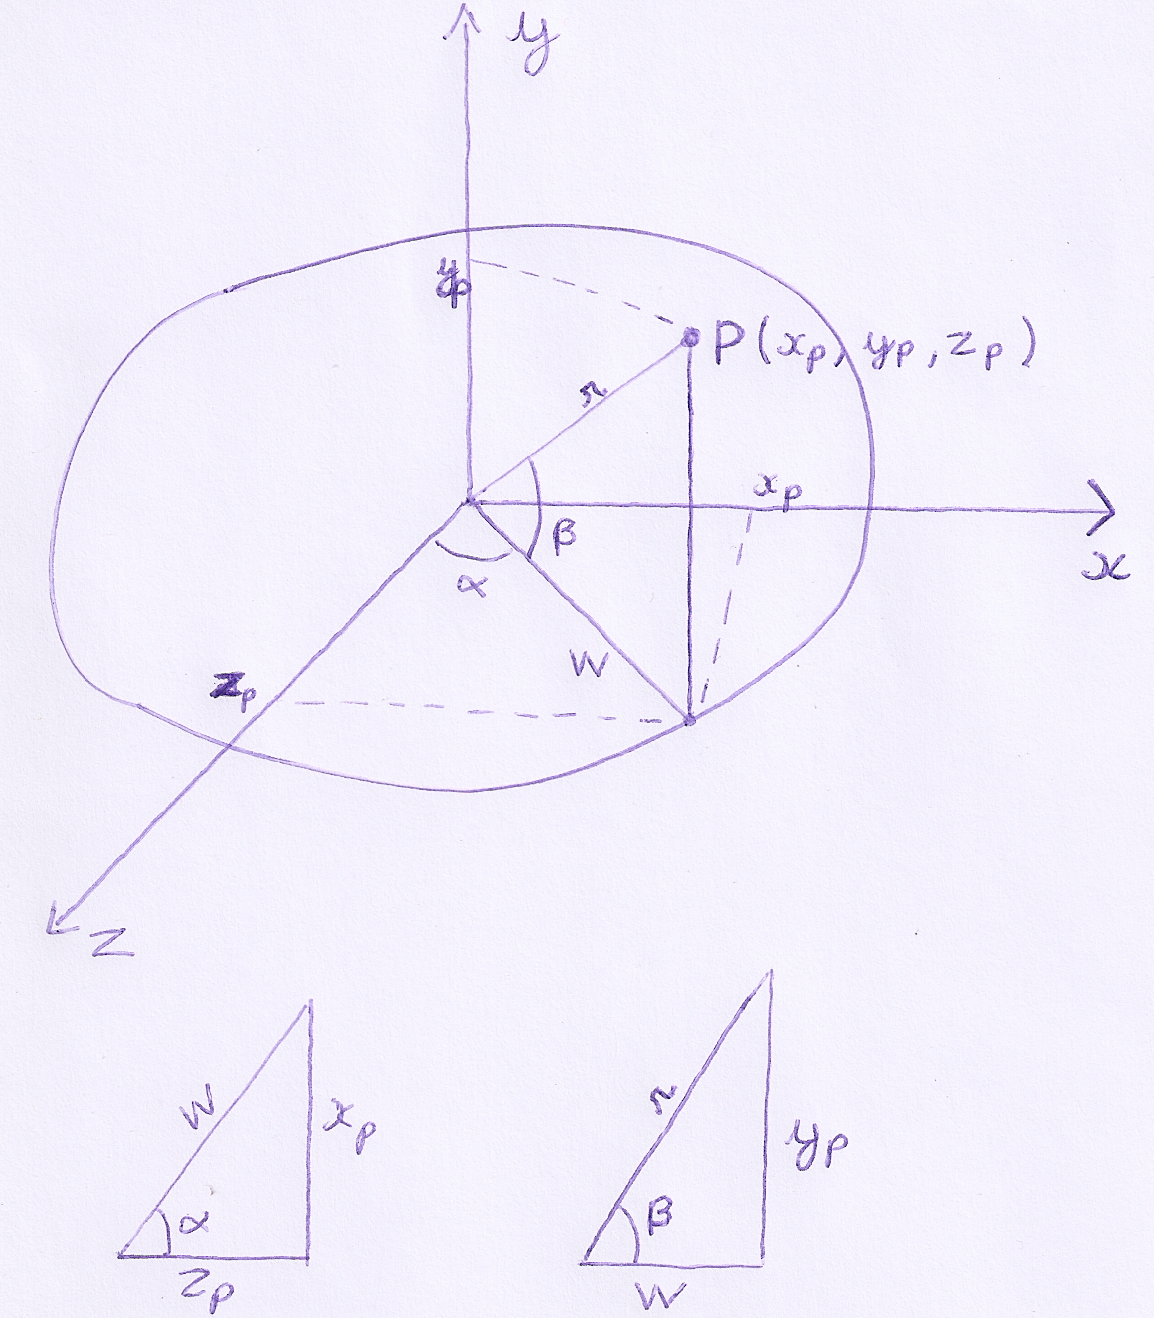
\includegraphics[height=12cm]{scan.png}
\end{figure}
%colocar imagem/figura e equações de modo a realizar a conversão
Sendo assim os valores das coordenadas cartesianas do ponto P bem como de w são:
\begin{itemize}
    \item $w = r * cos(\beta)$
    \item $x_{p} = r * cos(\beta) * sin(\alpha)$
    \item $y_{p} = r * sin(\beta)$
    \item $z_{p} = r * cos(\beta) * cos(\alpha)$
\end{itemize}

\subsection{Vertex Buffer Objects (VBOs)}
Numa fase inicial do trabalho foi tomada a decisão de ler o ficheiro XML a cada chamada da função \texttt{renderScene}, ou seja, no pior dos casos, tantas vezes quanto o \textit{refresh rate} do monitor. Isto representava no entanto um grande \textit{bottleneck} em casos em que o ficheiro fosse de tamanho considerável e os modelos em causa complexos. Para limitar este comportamento recorreu-se ao uso de \texttt{arrays} que armazenam as coordenadas de cada ponto sendo que cada modelo, representado por um conjunto de pontos, se encontra armazenado numa estrutura do tipo \texttt{modelPoints}.
Os modelos encontram-se armazenados numa lista ligada que é percorrida na fase de renderização. Nesta altura são usados VBOs que permitem armazenar os dados para renderização na memória do GPU ao invés da memória central apresentando, por isso, ganhos de performance significativos em relação à renderização imediata.

\begin{Verbatim}
    glBufferData(GL_ARRAY_BUFFER,(auxM->size)*3*sizeof(float),auxM->points,GL_STATIC_DRAW);
    glDrawArrays(GL_TRIANGLES,0,auxM->size);
    auxM = auxM->next;
\end{Verbatim}

\newpage

\section{Conclusão}
Tendo em conta o trabalho realizado e o uso de VBO's de modo a desenhar os pontos fica por realizar a validação dos parâmetros passados como input ao \textit{Generator} nomeadamente a verificação da positividade do número de slices e stacks do cone. 
É de destacar o ficheiro \textit{solarSytem} que especifca uma cena que representa o sistema solar. Optamos também por implementar o modo de visualização \textit{First Person Camera} que adiciona um maior realismo ao programa. Dos aspetos a melhorar no trabalho realizado destaca-se a verificação da sintaxe do ficheiro XML em relação à sua correção. 
Para além disso, foi realizado os Bezier Patches bem como a translação usando Catmull Rom e a rotação de 360º durante algum tempo. Contudo, possíveis melhorias passariam pela verificação de sintaxe dos ficheiros \textit{.patch}, algo que não é realizado, sendo que o generator assume que o ficheiro tem a sintaxe correta e, desta forma, quando não a tem o resultado é inesperado. Para além disso, poderiam ser adicionadas rotações também aos planetas e luas, algo que de momento só é realizado no Sol.

\newpage

\section{Referências}
stackoverflow.com/questions/7687148/drawing-sphere-in-opengl-without-using-glusphere
\newline
cpp.libhunt.com/compare-tinyxml2-vs-libxml2
\newline
www.xmlsoft.org/html/index.html
\newline
www.xmlsoft.org/html/libxml-tree.html
\newline
www.xmlsoft.org/html/libxml-parser.html
\newline
solar.physics.montana.edu/spot/teacher\_area/Scale\_Model\_Solar\_System\_Activity(6-8)
\newline
http://homepages.inf.ed.ac.uk/rbf/CVonline/LOCAL\_COPIES/AV0405/DONAVANIK/bezier.html
\newline
http://web.cs.wpi.edu/~matt/courses/cs563/talks/surface/bez\_surf.html

\end{document}
